\documentclass[manuscript, screen, review]{acmart} %removing review removes the numbers on left side
% \documentclass[sigconf]{acmart}

\AtBeginDocument{%
  \providecommand\BibTeX{{%  
    \normalfont B\kern-0.5em{\scshape i\kern-0.25em b}\kern-0.8em\TeX}}} %chktex 1

\usepackage{etoolbox} 
\apptocmd{\sloppy}{\hbadness 10000\relax} {}{} %chktex 1

\usepackage[skip=6pt plus1pt]{parskip} %% add space between the paragraphs

\usepackage{graphicx} %% For pictures
\graphicspath{{./pics/}}
\usepackage[section]{placeins} %% used to keep the images in the section that I want them in

\setcopyright{acmcopyright}
\copyrightyear{2024}
\acmYear{2024}
\acmDOI{XXXXXXX.XXXXXXX}

\begin{document}

\title{Music Versus No Music Effectiveness On Cognitive Response Time and Typing Efficiency}

\author{Jonquill Howlett}
\email{jonquill.howlett@colostate.edu}
\affiliation{%
  \institution{Colorado State University}
  \city{Berthoud}
  \state{Colorado}
  \country{USA}
  \postcode{80513-0650} %chktex 8
}

\author{Shea Spalding}
\email{Shea1@colostate.edu}
\affiliation{%
  \institution{Colorado State University}
  \city{Fort Collins}
  \state{Colorado}
  \country{USA}
  \postcode{80521-1873} %chktex 8
}

\renewcommand{\shortauthors}{Howlett, Spalding}
% the template does not show any shortauthors

\begin{abstract}
The abstract does not get added until after the project is finished or nearly finished.
\end{abstract}

\ccsdesc{Music, Typing Efficiency} % Update this
\keywords{Typing Efficiency with Music, Cognitive Function} % placeholder text for the time being
\maketitle

\section{Introduction}
This project will focus on people's ability to type with distractions such as different types of music playing. 
It will then test their cognitive ability to focus on a hand/eye coordination test in which we will test how well they can match shapes by measuring speed and accuracy. 
The two-part test aims to help test if the music is too distracting or will help the people be more efficient at their work. 
This is important because many people do their homework or jobs while listening to music and should they make a mistake, it could end up costing someone their grade or the mistake at work has a cascading effect to cause more errors in their work. 
The two-part test will help determine if there is a correlation between the effectiveness of music versus no music on cognitive response time and typing efficiency.

\subsection{Eye Tracking}
Eye tracking technology, such as the EyeWriter 2.0, has become increasingly valuable in cognitive research, allowing for precise measurement and analysis of visual attention and eye movements. 
In this study, we incorporate the EyeWriter 2.0 to track participants' eye movements during the QBTest, a hand-eye coordination task.
The EyeWriter 2.0 offers high-resolution tracking, capturing gaze patterns and fixations with accuracy. 
By analyzing participants' eye movements during the QBTest under different music conditions, we aim to understand how distractions, such as music, influence visual attention and cognitive performance.
Understanding the impact of music on cognitive response time and typing efficiency, as measured by the QBTest and eye tracking, can provide valuable insights for improving work and study environments where music is commonly used as a background stimulus.

\subsection{QBTest}
The Quantified Behavioral Test (QBTest) is a well-established tool for assessing cognitive function, particularly in measuring hand-eye coordination, speed, and accuracy.
Developed as a standardized measure, the QBTest provides valuable insights into cognitive performance across different tasks and conditions. % This would be a good place to put a citation.
In this study, the QBTest serves as a central component for evaluating participants' cognitive response time and typing efficiency under various music conditions.
By administering the QBTest alongside eye tracking using EyeWriter 2.0, we aim to understand the impact of music on cognitive function and task performance.
The QBTest's ability to quantify cognitive performance makes it an ideal tool for this study, allowing us to measure the effects of music on participants' ability to focus, process information, and perform tasks accurately. 
Through this research, we seek to provide insights that can enhance our understanding of how environmental factors, such as music, influence cognitive processes.

\subsection{Typing Test}
Typing proficiency is a fundamental skill in today's digital age, essential for academic and professional success. 
However, various factors can influence typing efficiency, including environmental stimuli such as music. Understanding how music affects typing speed and accuracy is crucial for optimizing work and study environments.
This study uses a typing test to assess participants' typing performance under different music conditions. 
The test presents participants with lyrics from popular songs, simulating a real-world typing scenario where individuals may listen to music while working or studying.
By measuring typing speed and accuracy under conditions of music with lyrics, music without lyrics, and no music (silent condition), we aim to determine the impact of music on typing efficiency. 
This research will contribute to our understanding of how environmental factors, such as music, can affect cognitive processes related to typing and may have practical implications for improving productivity in various settings.


\section{Related Works}
\subsection{Music While Working}
While there is not necessarily a concrete answer for whether music or background noise is effective on cognitive function, there have been many
studies that attempt to determine the answer. 
The other studies attempted to search for this answer by focusing on word processing on a computer with the background music and the user's ability to formulate sentences~\cite{ransdell2001141}, or determining if background music helps users to keep their attention on their task at hand~\cite{kiss2021effect}. 
Similar to Kiss and Linnell~\cite{kiss2021effect}, Mathew ~\cite{mathew2022inherently} also examined how motivation and music were used hand-in-hand on ``a time-consuming task and task performance''. 
A different study done in 2010 again found similar results of music both being a hindrance and benefit~\cite{AudioDistractionsAshley}. 
According to Gonzalez and Aiello~\cite{Gonzalez_Aiello_2019}, the degree of cognitive function may be based on an individual's personality. 
Furnham et al., also determined this was based on personality in a study done between extraverts and introverts although ``no significant interactions were found''~\cite{distractingEffectsFurnham}.

The research done by Komlao found that music or background music was again based on an individual's personality but that music, even music that the participants were familiar with, were a distraction and ``was found to negatively impact task performace'' overall~\cite{komlao2018variations}.
This was contrary to the previous studies found by Komlao where the ``music could help increase productivity for simple, monotonouse tasks''~\cite{komlao2018variations}.

Although Ransdell and Gilroy~\cite{ransdell2001141} suggests that the music is a detriment, those with ``musical training and high working memory span wrote better essays with longer sentences''. 
This suggests that while the music slowed down the participants, it did not necessarily lower their cognitive ability in typing on their computer while focusing on forming text for the written essay for this particular study. 
For Silverberg~\cite{AudioDistractionsAshley}, the music caused enough of a difference in the time that was taken for writing a paragraph but ``there were no significant differences in typing speed between the audio distractions''. 
This again may suggest that the participant's cognitive ability was not hindered when typing and may transfer directly after should the participants have taken a test measuring their cognitive function. 
The slow timing was again seen by Gonzalez and Aiello~\cite{Gonzalez_Aiello_2019} in which ``music generally impaired performance on a complex task but improved performance on a simple task''. 

The study done through Kiss and Linnell~\cite{kiss2021effect} saw opposite results as to Gonzalez and Aiello~\cite{Gonzalez_Aiello_2019}. The music or background noise ``enhanced'' the reaction time and performance of the tasks that are given to be completed. 
The results from Mathew~\cite{mathew2022inherently} were split. 
The music was a detriment for logic puzzles in the user's accuracy but aided in the efficiency of a writing task. 
According to Bramwell-Dicks et al., the instrumental music used in their study had better results on typists in speed and accuracy whereas music with vocals, the participants fared worse~\cite{bramwell2016can}.
While only a quasi-experiment, Oldham et al., found that personal headphones and Walkmans for employees had a postive correlation if the job complexity was not complex but also that employee satisfaction at this company was higher if they were allowed to use their walkman while working~\cite{oldhamListen}. Dobbs et al., also found the correlation that while music produced lower scores than silence it was better than just ``noise''~\cite{effectsOfBackgroundDobbs}.

\subsection{Eye Tracking and Quantified Behavioral Test}
% Citations about eye tracking and QBTest here

\section{Methodology}
After obtaining consent from all participants, they proceeded to take the typing test. The test presented lyrics from popular songs within a graphical user interface (GUI). 
The interface automatically calculated typing accuracy and the time the attempt took in the program's backend, allowing participants to focus solely on completing the test.
Each participant completed the typing test under three conditions: music with lyrics, music without lyrics, and no music (silent condition).
Multiple levels of music intensity were utilized within each condition to assess varying degrees of distraction.
The GUI of the typing test was built with simplicity in mind. The starting window was pulled up so as not to confuse participants with the code as seen in Figure 1. The participants saw Figure 2 while the test is running, while Figure 3 is the signifier that the typing portion is finished. 

\begin{figure}
  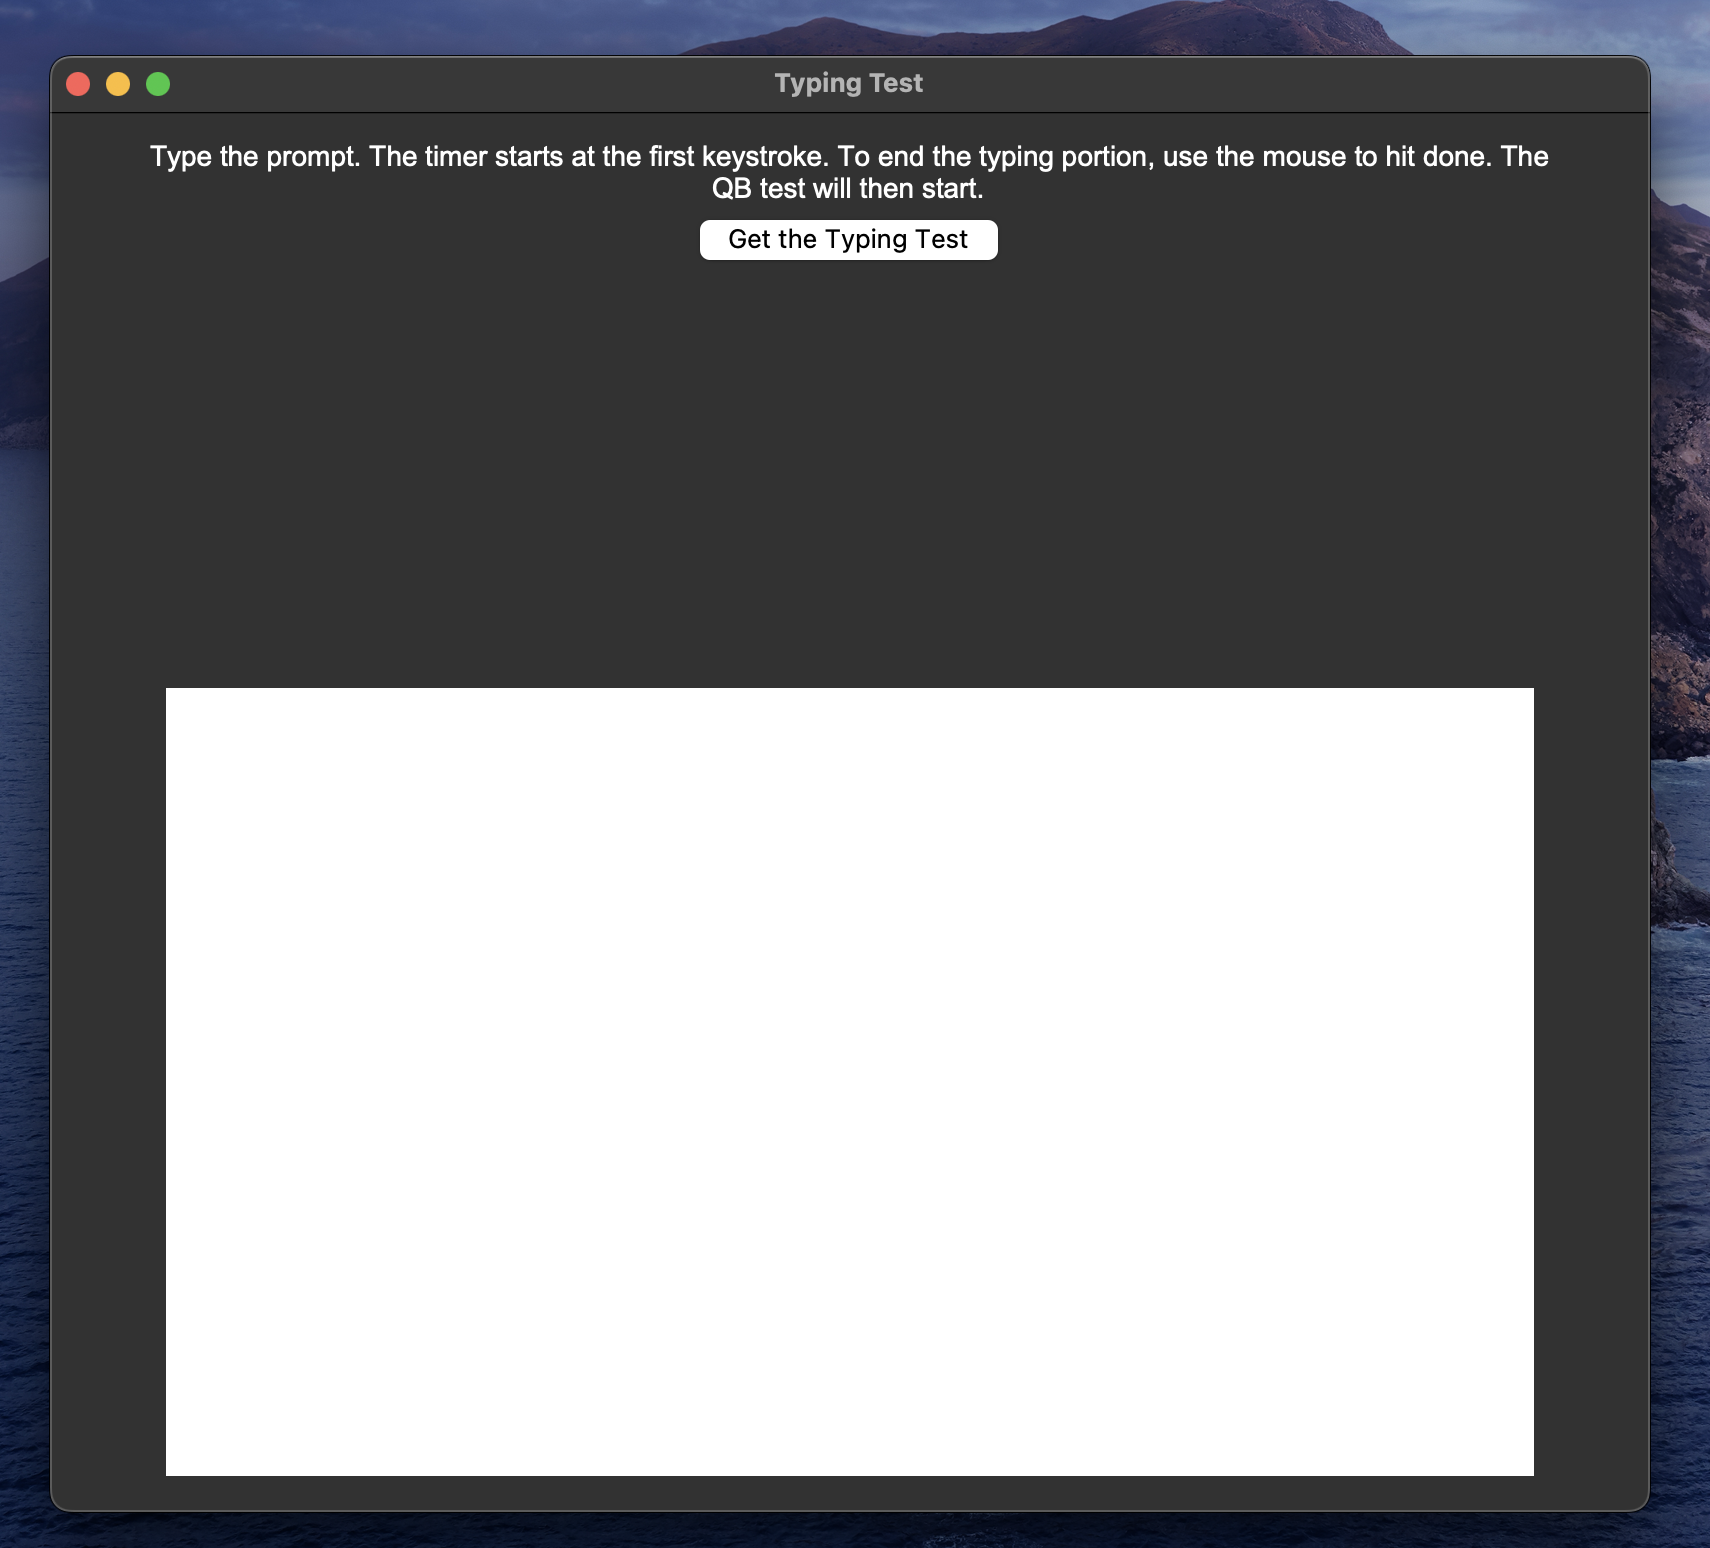
\includegraphics[width=0.3\textwidth]{typing_test_1}
  \caption{Starting window of typing test}
  \Description{Image of the starting windows of the typing test}
\end{figure}

\begin{figure}
  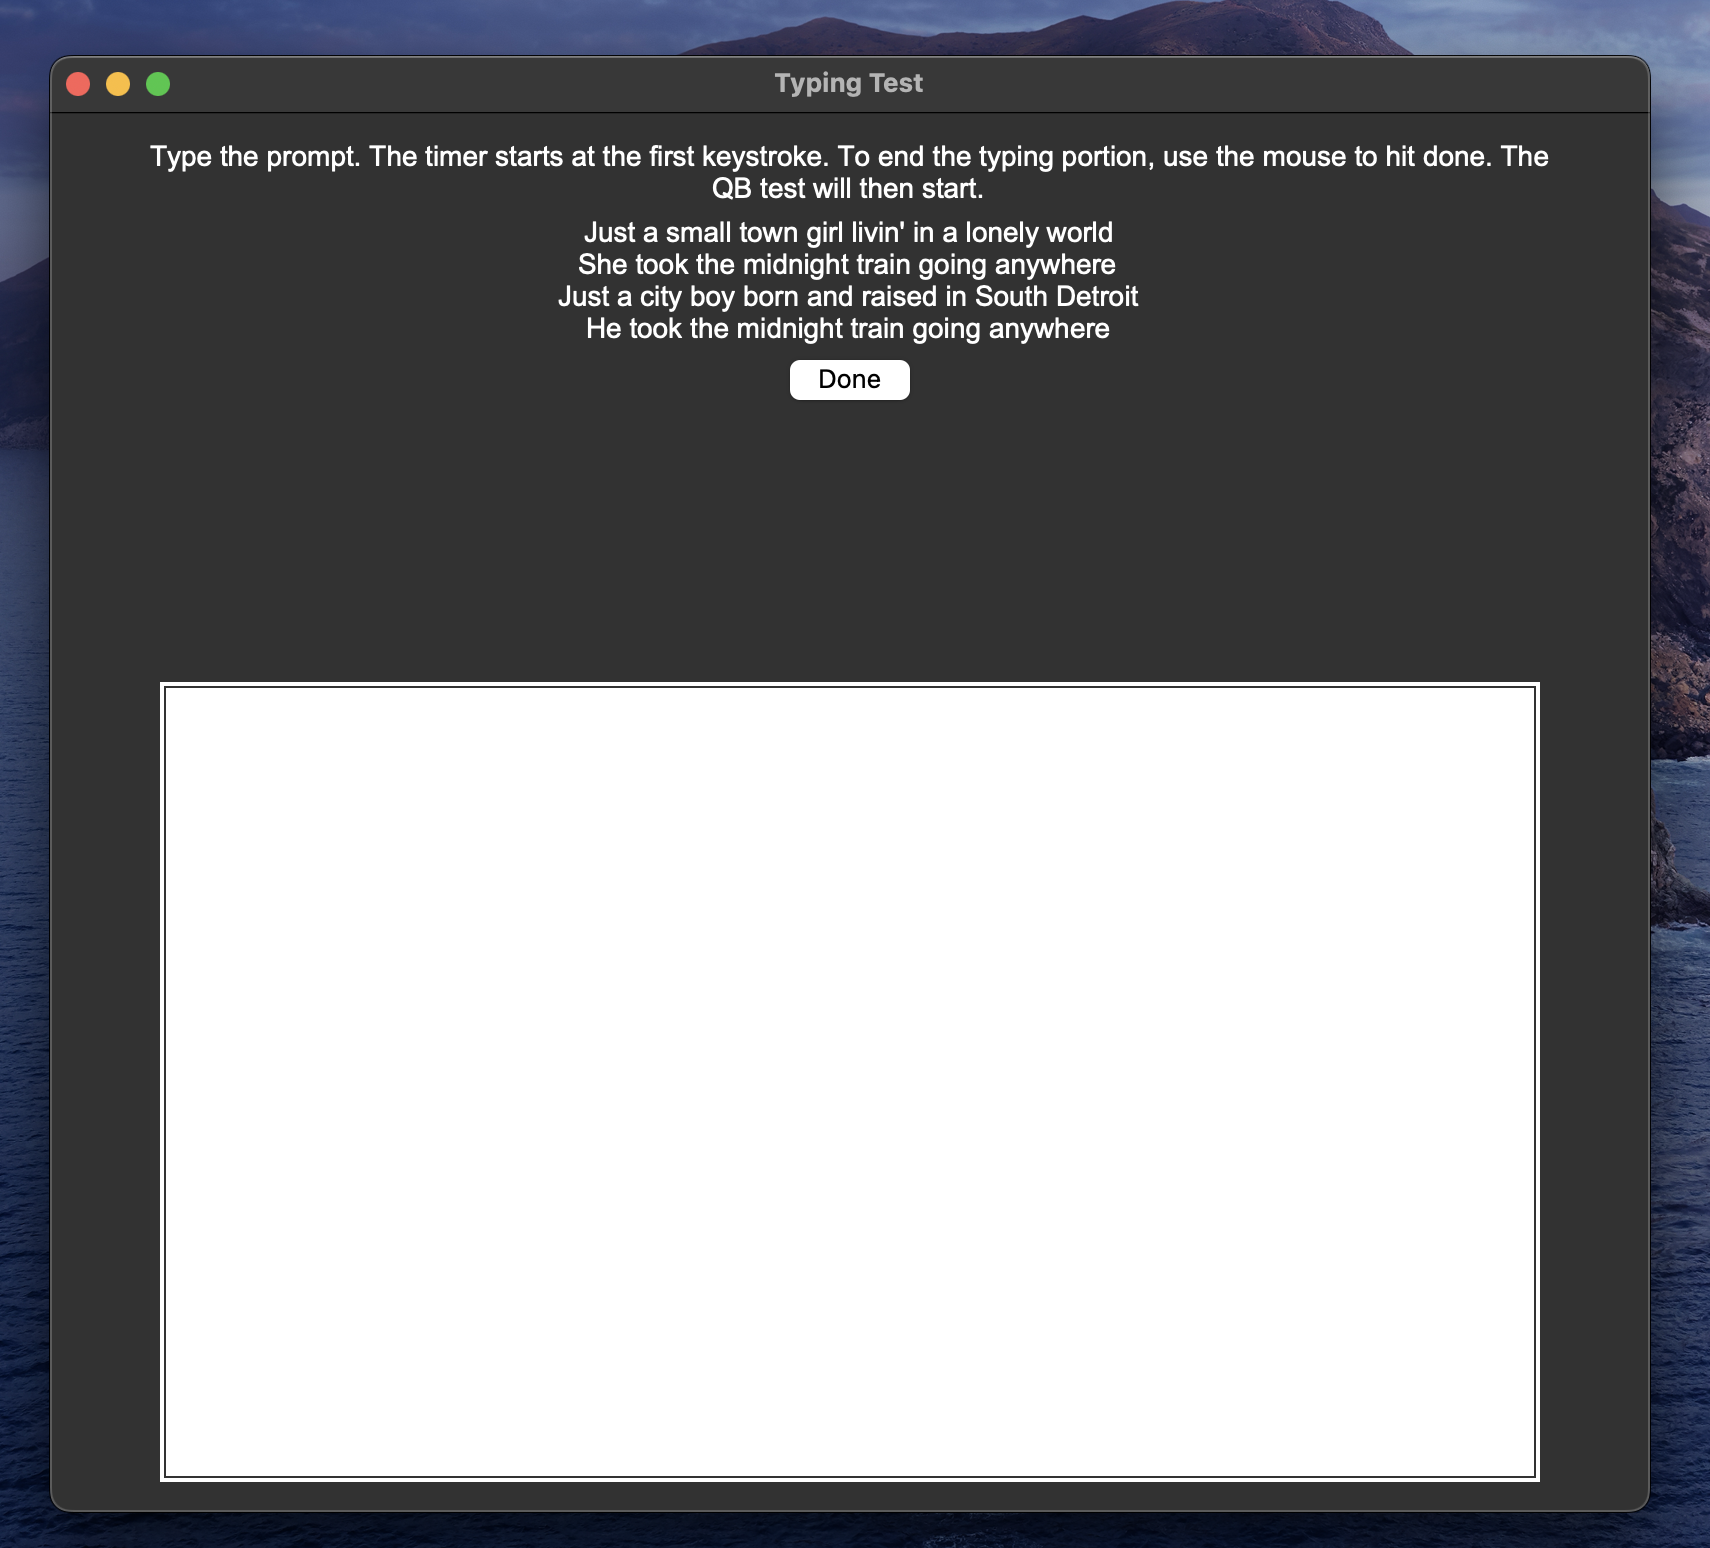
\includegraphics[width=0.3\textwidth]{typing_test_2}
  \caption{Test started}
  \Description{Image of the test with the lyrics that the user will type}
\end{figure}

\begin{figure}
  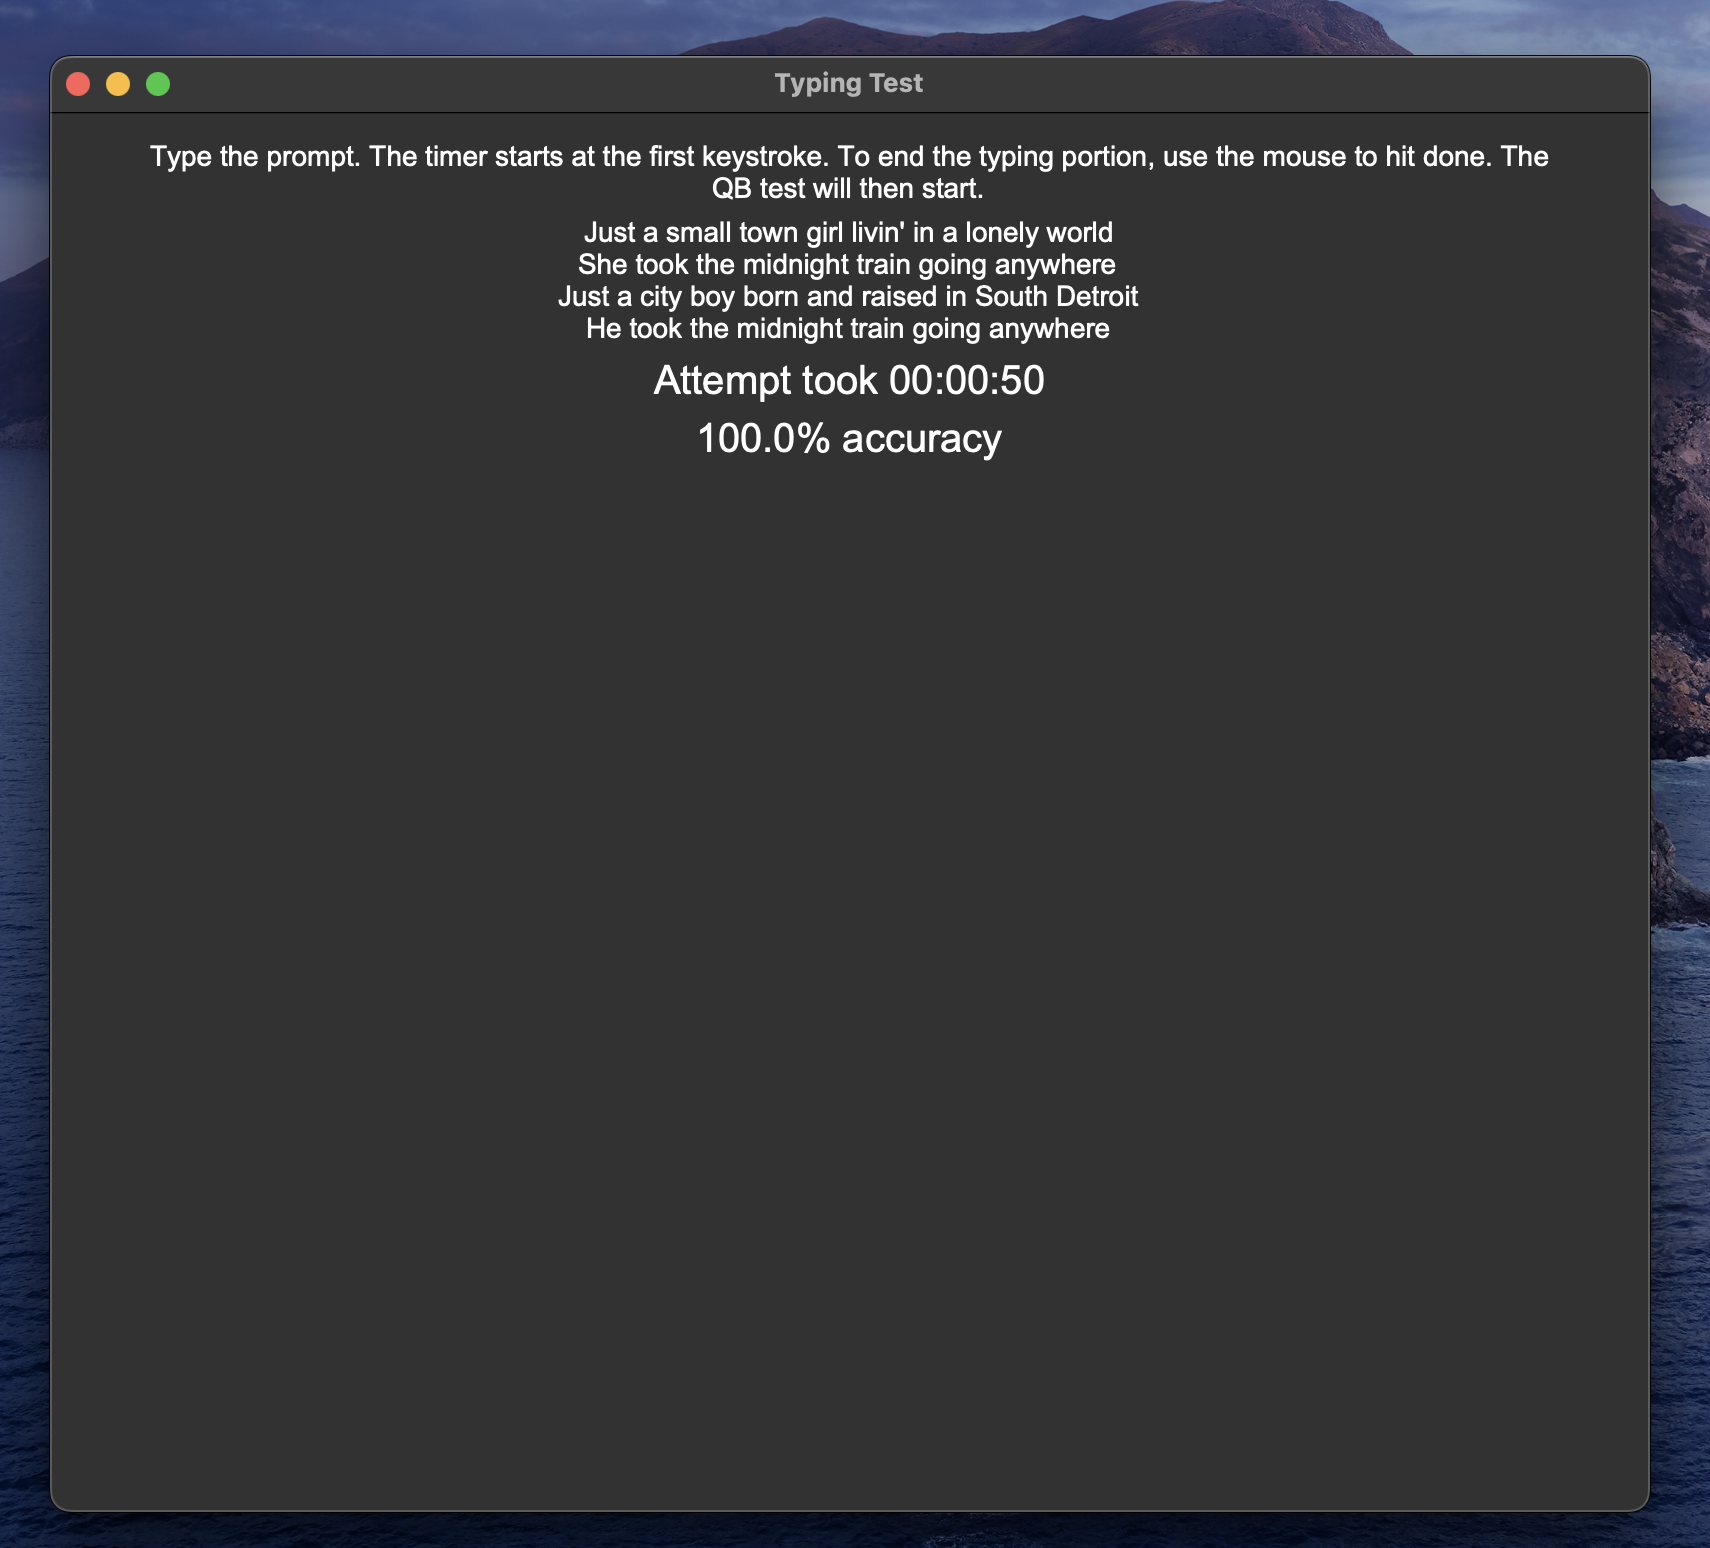
\includegraphics[width=0.3\textwidth]{typing_test_3}
  \caption{Test finished}
  \Description{Image of the finished test}
\end{figure}

They were given the instructions in the GUI with the text area where their text is clearly visible and the only button in the window to start the test and timer. 
After they hit the ``Get the Typing Test'' button, the lyrics of the randomly selected songs were displayed for the user to type. 
The text box for the users was already in focus with a ``Done'' button. After the users hit ``Done'', their accuracy and speed were presented.

Following the typing test, participants proceeded to the cognitive task component of the study, which was also conducted under the three aforementioned conditions. 
While the participants did the cognitive task of a quantified behavioral test, their eye movement will be tracked by the EyeWriter 2.0 camera that we specially built for this study. 
The EyeWriter system consists of a camera mounted on the participant's laptop, which tracks eye movements and allows for precise measurement of gaze direction and fixation duration.

Participants were seated in a comfortable position facing the laptop screen.
The laptop is placed on top of a laptop stand while the eye tracker is mounted on a wooden frame. 
While the eye tracker is on a moveable slider, it is centered in front of the screen. 
At the ends of the wooden frame are infrared lights that flashes at sixty frames per second. % will need to verify that it is 60 fps.
Although not pictured, a bluetooth keyboard is used by the participant for the quantified behavioral test (QBTest).

\begin{figure}
  \includegraphics[width=0.3\textwidth]{eyetracker_setup.png}
  \caption{EyeWriter 2.0}
  \Description{Image of the eye tracker setup}
\end{figure}

During the cognitive task component of the study, participants performed a Quantified Behavioral test or QBTest while their eye movements were tracked by the EyeWriter 2.0.
The QBTest is a computerized test designed to assess various aspects of cognitive function, including attention, impulsivity, and response control.
% Further details on the cognitive task will be provided in subsequent sections. They will then move on the the QBTest?. % This will need to be re-written.

\subsection[short]{Participants}
Tweleve participants were recruited from Colorado State University or Fort Collins, Colorado. NUMBER males and NUMBER females all in the age range of 18-99. There were no %chktex 8
restrictions in regards to their major as long as they were able to type on a keyboard with no tilt on the keys.
They have all previously either learned to type at primary school or through necessity.

\subsection[short]{Equipment} 
% This may not need to be broken into subsections. Will decide before we resubmit. 
Participants used two different MacBook Pros in this study due to the nature of the eye tracker setup although both were running on Sonoma or MacOS 14. One MacBook Pro was used to administer the QBTest, and it had the eye tracker mounted on it. The positioning of the eye tracker made it challenging to use this MacBook Pro for the typing test and QBTest. 

QBTest MacBook Pro with Eye Tracker: This MacBook Pro was dedicated to conducting the QBTest. It had the eye tracker mounted on it, which made it difficult to access the keyboard for typing. Participants used this MacBook Pro for the QBTest to ensure that the eye tracker could accurately track their eye movements during the test. A bluetooth keyboard was used as part of the QBTest since the positioning of the Eye Writer mostly blocked the space bar.

Typing Test MacBook Pro: The second MacBook Pro was used for the typing test. Since it did not have the eye tracker mounted on it, participants could easily access the keyboard and perform the typing test without any interference from the eye tracker.
Using two separate MacBook Pros allowed for the independent administration of the QBTest and typing test, ensuring that participants could perform each task without any physical hindrance from the eye tracker.

\subsubsection{EyeWriter 2.0}
The IR camera captures the eye movements of the participant.
It is mounted on the laptop that participants use for the QBTest, allowing for the tracking of eye movements during the test.
IR LEDs are used to illuminate the eye to enhance the visibility of the eye for tracking purposes. 
These LEDs are also mounted on the laptop along with the IR camera. 
The mounting system holds the IR camera and IR LEDs in place relative to the participant's eye. 
It ensures that the camera has a clear view of the eye for accurate tracking. 
Cables are used to connect the IR camera and IR LEDs to the laptop. These cables transmit data and power between the components.
An Arduino microcontroller allowed the computer to communicate with the camera, infrared LED lights, and computer.

\subsubsection{Typing Test}
The typing program was written in Python and compiled using Python3.9. 
While python can run on any device that has python installed, this study only used the two Macbook Pros. 
The singularity of the devices was used as the center of the screen for the typing test was hard coded when setting the starting position of the window for the typing test. 

\subsubsection{Quantified Behavioral Test}
The Quantified Behavioral Test program was written in Python and compiled using Python3.9.
The package pygame was used for this interface compared to the package tkinter used for the typing test.
The bluetooth keyboard allowed the participant to hit the space bar when the QBTest said to hit the space bar.

\subsection[short]{Procedure}
Each participant was instructed to read and then sign the consent form. While the consent form had the basis of what they would be doing, they were given more detail as to the instructions when they were ready to begin.
 %REWRITE THIS HERE
%First they would take the short typing test three times to account for the three levels of music. 
%They would then do a QBTest three times again for the music. 
%The eye tracker is mounted around a laptop stand and the laptop is placed in between the stand so that the screen is behind the eyetracker.
The two computers were set up side by side so that it would be easy for the participant to switch between the typing test and QBTest.
This setup also made it simple for the music component as the participants did each level together (e.g. the no music level was typing test 
then the QBTest) before moving on to the next level.

\subsection[short]{Design}
Design

\section{Results and Discussion}
Within-subjects testing was used.

\section{Conclusion}
Conclusion

\bibliographystyle{ACM-Reference-Format}
\bibliography{paper}

\end{document}
